\subsection{Cargas}
\noindent La carga es una unidad cuantizable, a partir de la carga del electrón \(e^{-}\),  siendo posible la carga una unidad de magnitud positiva o negativa. \par \noindent
Esta unidad afecta a nivel de la Fuerza Electrostática, el Campo Electrostático y sus magnitudes, y podemos considerar que todas las cargas poseen masa. \par \noindent
Además, dado un sistema, siempre \underline{la suma de todas las cargas va a ser cero}. De este enunciado podemos decir dos principios:
\begin{itemize}
        \item \underline{Principio de Conservación de la Carga}: La suma de todas las cargas del Universo vale cero, es decir, la carga total es \(\bm{cte}\)
        \item \underline{Principio de Conservación local de la Carga}: La suma de todas las cargas en un sistema, es \(\bm{cte}\) es decir, vale 0.
\end{itemize}
\subsection{Ley de Coulumb}
\noindent Esta es la ley fundamental que describe la interacción entre dos cargas puntuales en un medio, independientemente del tamaño del cuerpo. Consideramos la carga total del sistema, y no la unitaria por cada sección del cuerpo. \par
\hspace{4cm}
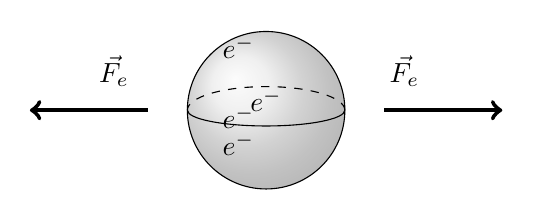
\begin{tikzpicture}
        \shade[ball color = gray!40, opacity = 0.4] (0,0) circle (1cm);
        \draw (0,0) circle (1cm);
        \draw (-1,0) arc (180:360:1 and  0.2);
        \draw[dashed] (1,0) arc (0:180:1 and 0.3);
        \node[left = 10, above = -20]{\(e^-\)};
        \node[left = 0, above = -4]{\(e^-\)};
        \node[left = 10, above = 15]{\(e^-\)};
        \node[left = 10, above = -10]{\(e^-\)};
        \node[right = 50, above = 5]{\(\vec{F_e}\)};
        \draw[->,ultra thick] (1.5,0)--(3,0);
        \node[right = -55, above = 5]{\(\vec{F_e}\)};
        \draw[->,ultra thick] (-1.5,0)--(-3,0);
\end{tikzpicture} \par
\noindent Cada cuerpo generará su propio campo y si consideramos las cargas puntuales, la fuerza entre ambas cargas será:
\[
        \boxed{\vec{F_{12}} = K \hspace{1mm}\frac{q_1q_2}{\left | \vec{r_2} - \vec{r_1} \right |^2}\hspace{2mm}\hat{r} = K \hspace{1mm}\frac{q_1q_2}{\left | \vec{r_2} - \vec{r_1} \right |^3}\hspace{2mm}(\vec{r_2} - \vec{r_1}) \hspace{3mm}N} \hspace{.25cm}
        \substack{\textnormal{\scriptsize{Siendo esta, el vector fuerza que ejerce la carga}} \\
                \textnormal{\(q_1\) sobre la carga \(q_2\).}}
\]
\[
        \boxed{\vec{F_{12}} = -\vec{F_{21}}} \hspace{.25cm}
        \substack{
                \textnormal{\scriptsize{Y evidentemente, el vector fuerza que ejerce la carga \(q_2\) sobre la carga \(q_1\) }}\\
                \textnormal{\scriptsize{es opuesta al vector fuerza que ejerce la carga \(q_1\) sobre la carga \(q_2\)}}
        }
\]
\newline
De esta forma podemos concluir con lo siguiente.
\begin{itemize}
        \item Las cargas de igual signo se repelen, mientras que las de signo diferente se atraen.
        \item Los vectores de posición son respecto a un punto de referencia. Siendo \(\bm{\vec{r_2}}\) el vector del punto destino, y \(\bm{\vec{r_1}}\) el vector del punto de partida.
        \item \(\bm{K}\) es la constante de Couloumb en el vacío y es lo mismo que \(\bm{K = \frac{1}{4\pi\epsilon_{\textnormal{o}}}}\), siendo \(\bm{\epsilon_{\textnormal{o}}}\) la permitividad en el vacío.
\end{itemize}
\subsection{Campo Electrostático}
\noindent El campo es la manifestación de la perturbación en el espacio generado por una carga puntual:
\[
        \boxed{\vec{E} = \hspace{1mm}\frac{\vec{F_e}}{Q} \hspace{1mm}= \hspace{1mm} Kq\frac{\vec{r} -\vec{r`}}{\left | \vec{r} -\vec{r`} \right |^3} \hspace{3mm}V/m} \hspace{1cm}
        \substack{\textnormal{Siendo \(\vec{r`}\) el vector entre el punto de referencia y la carga y }
                \\
                \textnormal{\(\vec{r}\) es el vector entre el punto de estudio y el punto de referencia}
        }
\]
\\
Solo podemos calcular el campo cuando la carga \(\bm{q}\) es muy pequeña, o lo que es lo mismo: \(\bm{\lim_{q \to 0} \vec{E} \approx 0}\) \par
\vspace{0.5cm}
\noindent Sabiendo como se expresa el campo electrostático, nos interesaría conocer algunos casos puntuales dignos de consideración:
\begin{itemize}
        \item Dado un plano con dos cargas puntuales en el mismo eje de coordenadas, y queriendo calcular el campo en un punto cualquiera a una distancia equidistante respecto a las dos cargas es igual a:
              \begin{itemize}
                      \item \(\vec{E_x} = \bm{2\left | \vec{E} \right | \cos{\bm{\alpha}}}\hspace{2mm} \bm{\hat{\imath}}\)
                      \item \(\vec{E_y} = \bm{2\left | \vec{E} \right | \sin{\bm{\alpha}}} \hspace{2mm} \bm{\hat{\jmath}}\)
              \end{itemize}
        \item Las cargas actúan como sumideros.
        \item El campo generado por una carga eléctrica se emite de forma radial y constante, y su número indica su intensidad.
\end{itemize}
\subsection{Distribución de Cargas}
\noindent Hemos considerado un cuerpo cualquiera con carga, como una carga puntual que genera un \(\bm{\vec{E}}\), ya que la carga se distribuía de forma continua. Sin embargo en la realidad no es así, y dependiendo del cuerpo que tengamos, su forma y tamaño afectarán al cálculo del campo. Para esto, deberemos calcular sección por sección del cuerpo de estudio con el fin de obtener una aproximación del campo total. En esta parte veremos \underline{la distribución de cargas por unidad de longitud} que la denotaremos por:
\[ \boxed{\lambda = \frac{Q}{l}} \hspace{2cm} \textnormal{Siendo \(\bm{Q}\) la carga y \(\bm{l}\) la unidad de longitud.}\]
Estudiaremos un caso muy particular, el campo generado por una barra metálica \\ infinítamente larga.\par
\vspace{0.5cm}
\hspace{4.5cm}
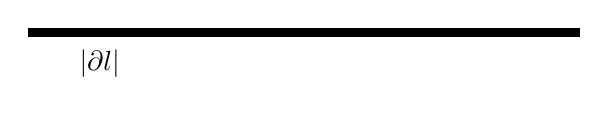
\begin{tikzpicture}
        \node[above = -10, right =15]{\(\left | \partial{l} \right |\)};
        \draw[draw=black, fill=black] (0,0) rectangle ++(7,0.1);
\end{tikzpicture}
\vspace{0.5cm}
\[
        \boxed{\vec{E}(P) \hspace{1mm} = \hspace{1mm}\frac{1}{4\pi\epsilon_o}\int^{b}_{a} \lambda \frac{\hat{r}}{r^2}\hspace{1mm} \mathrm{d}l \hspace{1mm} = K\lambda \int^{b}_{a}\frac{\vec{r}}{r^3} \mathrm{d}l\hspace{1mm} = K\lambda \int_{a}^{b} \frac{y}{h}\vec{\jmath} -\frac{x}{h} \vec{\imath} \hspace{2mm}\mathrm{d}l}
\]
Siendo \(\bm{h = \sqrt[]{x^2+y^2}}\) y las incógnitas \(\bm{x}\) e \(\bm{y}\) como la distancia de un punto cualquiera en la barra para las coordenadas X e Y respectivamente. Los valores \(\bm{a}\) y \(\bm{b}\) de la integral, no son más que dos extremos cualquiera de la barra cargada.
\subsection{Ley de Gauss}
\begin{wrapfigure}{r}{3cm}
        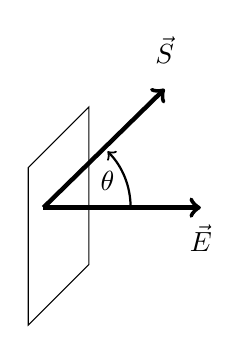
\begin{tikzpicture}[scale=2]
        \pgfmathsetmacro{\cubex}{2}
        \pgfmathsetmacro{\cubey}{1}
        \pgfmathsetmacro{\cubez}{1}
        \draw[] (0,0,0) -- ++(0,0,-\cubez) -- ++(0,-\cubey,0) -- ++(0,0,\cubez) -- cycle;
        \draw[->,ultra thick] (0,-.35,-0.25) --(1,-.35,-.25) node[above = -20]{\(\vec{E}\)};
        \draw[->,ultra thick] (0,-.35,-0.25) -- (30:1) node[above = 5]{\(\vec{S}\)};
        \draw[->,thick] (0.65,-.25) arc (0:45:0.5) node[above = -18]{\( \theta\)};
\end{tikzpicture}
\end{wrapfigure}
\noindent La ley de Gauss define el flujo de \(\bm{\vec{E}}\) a través de una superficie cerrada.\par
\noindent Podemos considerar un caso general, donde dado un espacio cualquiera, con tamaño y forma indefinidos el flujo del campo eléctrico se denota por:
\[
        \phi =\lim_{\Delta S \to 0}\sum_{i=0}^{\infty}\vec{E_i}\hspace{1mm}\Delta S = \int_{S}\vec{E}\hspace{1mm}\mathrm{d} \vec{S} = \boxed{\oint_{S} \vec{E} \hspace{1mm}\mathrm{d} \vec{S} = \frac{Q_\textnormal{int}}{\epsilon_o}}
\]
Dada esta expresión podemos deducir que el flujo total es la suma, infinitesimal de cada una de las secciones sobre la que ejerce el campo eléctrico sobre la superficie, y que el flujo \(\bm{\phi}\) es proporcional a la carga interna \(\Rightarrow \boxed{\bm{\phi} \hspace{1mm} \bm{\propto} \hspace{1mm} \bm{q}}\) \par
\vspace{1cm}
\hspace{-.5cm}
Por lo tanto podemos estudiar el valor del campo \(\bm{\vec{E}}\) en casos de extrema simetría.
Para esto consideraremos una nueva magnitud \(\bm{\sigma}\) que denota la \underline{distribución superficial de carga}. \(\boxed{\sigma = \frac{Q}{S}}\)
\par \vspace{.5cm} \hspace{-.5cm}No confundir la superficie del cuerpo de estudio con la superficie Gaussiana, esta es variable y depende de quien la estudie.
\subsubsection{Plano Infinito}
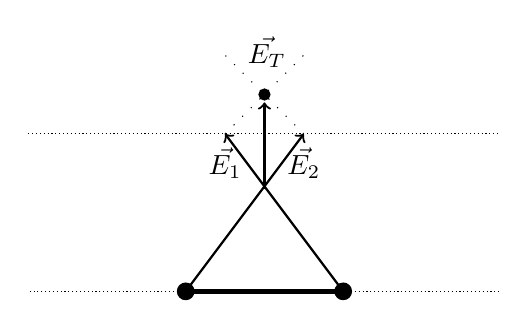
\begin{tikzpicture}
        \draw[densely dotted] (-2,2) -- (4,2);
        \draw[-,ultra thick] (0,0) -- (2,0);
        \draw[densely dotted] (2,0) -- (4,0);
        \draw[densely dotted] (0,0) -- (-2,0);
        \draw[->, thick] (2,0) -- (0.5,2) node[above = -20]{\(\vec{E_1}\)};
        \draw[->, thick] (0,0) -- (1.5,2) node[above = -20]{\(\vec{E_2}\)};
        \filldraw[color = black] (2,0) circle (3pt);
        \filldraw[color = black] (0,0) circle (3pt);
        \draw[loosely dotted] (0.5,2) -- (1.5,3) node[above = 1, left = 3]{\(\vec{E_T}\)};
        \draw[loosely dotted] (1.5,2) -- (0.5,3);
        \filldraw[color = black] (1,2.5) circle (2pt);
        \draw[->, thick] (1,1.3) -- (1,2.4);
\end{tikzpicture}\par
\noindent Dado el diagrama propuesto, todos los puntos situados en el mismo plano, poseen la misma \\Distribución Superficial de Carga, y por ende todos los puntos poseen el mismo \(\vec{E}\).
\[\vec{E} = \vec{E_1} + \vec{E_2} = 2\vec{E}\]
\subsubsection{Cilindro en un plano infinito}
\noindent Si situaramos un cilindro en un plano infinitamente largo, observamos que el flujo corresponde a la suma del flujo que pasa por cada una de las tapas y la cubierta lateral del cilindo. De esta forma, debido a que la cubierta lateral es paralela al vector normal al campo, el flujo que pasa por ahí es nulo. Por ende:
\[
        \oint \vec{E}\hspace{1mm}\mathrm{d} \vec{S} = \oint_{SL}\vec{E}\hspace{1mm}\mathrm{d} \vec{S} +\oint_{S^+}\vec{E}\hspace{1mm}\mathrm{d} \vec{S}+\oint_{S^-}\vec{E}\hspace{1mm}\mathrm{d} \vec{S} =
        2 \oint_{S^+} \vec{E}\hspace{1mm}\mathrm{d} \vec{S} \Rightarrow \phi =2\left | \vec{E} \right |\left | \vec{S} \right | = 2ES
\]
\[
        2ES = \frac{Q_{\textnormal{int}}}{\epsilon_o} \Rightarrow E = \frac{\left | \sigma \right |}{2\epsilon_o} \Rightarrow \boxed{\vec{E} = \frac{\sigma}{2\epsilon_o}\hspace{1mm}\hat{n}}
\]
Posteriormente veremos que si el cuerpo está cargado y analizamos el campo \(\bm{\vec{E}}\), este valdrá 0, y por tanto su potencial es \(cte\) aunque no sepamos cuanto pueda valer. \textbf{El vector \(\bm{\hat{n}}\) es el vector normal a la superficie}.
\subsubsection{Esfera cargada}
\noindent Aplicando la Ley de Gauss y considerando \(\bm{R}\) el radio de la superficie Gaussiana, y \(\bm{r}\) el radio de la esfera:
\[
        \oint \vec{E} \hspace{1mm} \mathrm{d}\vec{S} \Rightarrow \left | \vec{E} \right | 4\pi R^2 = \hspace{1mm} \frac{Q_{\textnormal{int}}}{\epsilon_o}
\]
\[
        \boxed{\vec{E}  = \hspace{1mm} \frac{Q_{\textnormal{int}}}{\epsilon_o4\pi R^2} \hspace{1mm}\hat{n} \hspace{1mm} = \frac{\sigma r^2}{\epsilon_o R^2} \hspace{1mm}\hat{n}}
\]

\subsection{Balance de Energías}
\begin{wrapfigure}{r}{5cm}
        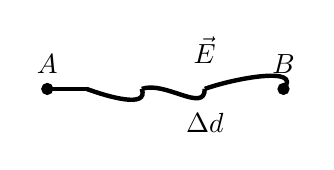
\begin{tikzpicture}
        \draw[-,ultra thick] (0,0) -- (0.5,0);
        \draw[-,ultra thick] (0.5,0) to[out=-20,in=-70] (1.2,0);
        \draw[-,ultra thick] (1.2,0) to[out=20,in=-90] (2,0) node[above =-20]{\(\Delta d\)} node[above =5]{\(\vec{E}\)};
        \draw[-,ultra thick] (2,0) to[out=20,in=50] (3,0);
        \filldraw[color = black] (0,0) circle (2pt) node[above =2]{\(A\)};
        \filldraw[color = black] (3,0) circle (2pt) node[above =2]{\(B\)};
\end{tikzpicture}
\end{wrapfigure}
\noindent Debido a que la fuerza electrostática es una fuerza conservativa, no importa la ruta recorrida, sino las posiciones inicial y final para calcular el trabajo requerido para mover la carga de un punto \textbf{A} al \textbf{B}.\par
\vspace{0.5cm}
\hspace{-.725cm}
De esta forma podemos aplicar \underline{El Teorema de las Fuerzas Vivas} por lo que \(\boxed{W_{A \to B} = \Delta E_c = \frac{1}{2} m (V_B -V_A) \hspace{2mm}J}\)
\par
\vspace{0.5cm}
\hspace{-.6cm}
Por lo tanto el trabajo requerido para mover una carga de un punto A a otro B, es igual a \(\ \Rightarrow \boxed{W_{A \to B} =-\Delta E_p = -q \Delta V}\) \par
\vspace{0.5cm}
\noindent Por convenio diremos que  \(\bm{E_c}\) es la energía cinética, \(\bm{E_p}\) es la energía potencial (ambas en Julios \textbf{J}) y \(\bm{V}\) es el potencial eléctrico, en Vatios \textbf{V}
\[
        \textnormal{En funcion del signo} \rightarrow
        \begin{cases}
                \textnormal{Si \(\bm{W > 0}\), \(\bm{q}\) se mueve a favor del campo} \\
                \\
                \textnormal{Si \(\bm{W < 0}\), \(q\) requiere de un \(\bm{W_{\textnormal{ext}}}\) para moverse.}
                \\
                \textnormal{Si la carga se queda quieta al recorrer ese trayecto, diremos que}
                \\
                \textnormal{\(\bm{W_\textnormal{ext} = -W}\)}
        \end{cases}
\]
\noindent Gracias al conocimiento del trabajo, podemos decir que las unidades del Campo Eléctrico pueden ser tanto \textbf{N/C} como \textbf{V/m}
\subsection{Superficies Equipotenciales}
\noindent Estos son aquellos espacios donde la diferencia de potencial \(\bm{\Delta V}\) vale siempre cero, es decir, tienen el mismo potencial en todos los puntos. \\
Los espacios que satisfacen esta situación son aquellos situados paralelamente, en sentido del campo eléctrico. \\ Es decir:
\[
        \boxed{\Delta V = E \mathrm{d} \cos{\alpha} \Rightarrow \mathrm{d}V = - \vec{E}\mathrm{d}\vec{r}}
\]
\begin{wrapfigure}{r}{5cm}
        \begin{tikzpicture}[scale=1]
        \draw[-,thick] (0,0)--(0,3) node[above = -110]{\(V_a\)};
        \draw[-,thick] (3,0)--(3,3) node[above = -110]{\(V_b\)};
        \draw[densely dotted] (-2,1) to[out=20,in=-50] (2,1) node[above = -21]{\(>\)};
        \draw[densely dotted] (2,1) to[out=30,in=10] (3.5,1);
        \draw[densely dotted] (-2,1.75) to[out=20,in=-50] (2,1.75) node[above = -21]{\(>\)};
        \draw[densely dotted] (2,1.75) to[out=30,in=10] (3.5,1.75);
        \draw[densely dotted] (-2,2.5) to[out=20,in=-50] (2,2.5)node[above = -21]{\(>\)};
        \draw[densely dotted] (2,2.5) to[out=30,in=10] (3.5,2.5);
        \node[right = 20, above = 10]{\(\bm{\vec{E}}\)};
\end{tikzpicture}
\end{wrapfigure}
Dada esta expresión, dos puntos son equipotenciales cuando \(\bm{\cos{\bm{\alpha}} = 0}\). Como se puede ver en el diagrama, todos los puntos paralelos, en función de las líneas de campo, son equipotenciales entre si.
\subsection{Conductores}
\noindent Las cargas en un conductor tenderán a moverse, mientras circula un campo \(\bm{\vec{E}}\), hasta que la carga neta del sistema se estabilice y quede en equilibrio, alrededor de unos \(10^{-14}\) segundos.\\\\
Estos materiales poseen una serie de propiedades, estudiandolos internamente, estas son:\\\\
\hspace{3cm}\textbf{Propiedades:}
\begin{enumerate}
        \item \(\bm{\vec{E}}\) en el interior es nulo (sino, las cargas no tenderían a equilibrarse)
        \item  El potencial es \(cte\) en todo el conductor, interior y superficie, es decir, todo el conductor es una superficie equipotencial.
        \item La carga neta tenderá a acumularse en la superficie del conductor, esto se puede demostrar con \underline{la Ley de Gauss}:
              \[
                      \boxed{\oint \vec{E} \mathrm{d} \vec{S} = \frac{Q_{\textnormal{int}}}{\epsilon_{\textnormal{o}}} \Rightarrow \vec{E} = 0 \Leftrightarrow  Q_{\textnormal{int}} = 0}
              \]
        \item El campo \(\bm{\vec{E}}\) en la superficie, hará que la carga se mueva a los bordes, por lo que \(\bm{\vec{E} \not \perp \vec{S}}\)
        \item \(\bm{\vec{E}}\) en la superficie vale \(\bm{\vec{E} = \frac{\sigma}{\epsilon_o}\hat{n}}\)
\end{enumerate}
\vspace{0.5cm}
En la realidad, un conductor no es completamente puro, no siempre, por lo que si este se encontrase en un campo eléctrico externo, \(\bm{\vec{E}}\) interna tenderá a cero, mientras que las cargas internas se moverán a favor del campo externo.
\subsubsection{Jaula de Faraday}
\noindent Son estructuras que son cargadas con carga eléctrica hasta el punto del \underline{Campo de Ruptura}, un estado en el cual el material servirá como aislante frente a campos eléctricos externos.
\subsubsection{Capacidad de un Conductor}
\noindent La expresión de la capacidad \(\bm{\mathcal{C}}\) que se mide en \textbf{Faradios}, \(\bm{F}\), no es más que el cociente entre la carga del sistema entre su potencial:
\[
        \boxed{\mathcal{C} = \frac{Q}{V}}
\]
Esta expresión se consigue a partir de la integración del potencial en un punto de la superficie del conductor, considerando que la \underline{distribución superficial de carga \(\bm{\sigma}\)} es igual al cociente entre la derivada de la carga y la superficie. Es decir:
\[
        \sigma = \frac{\mathrm{d}q}{\mathrm{d}S}
\]
\[
        V(p) = \int \frac{\sigma K}{r} \mathrm{d}S \approx Q = V \mathcal{C}
\]
\subsection{Condensador}
\noindent Un condensador es un elemento formado por dos conductores de influencia total, es decir, poseen la misma carga pero de signos distintos. Un caso particular es el condensador de placas planas y paralelas.
\newpage
\subsubsection{Condensador de Placas Planas y Paralelas}
\begin{wrapfigure}{l}{0cm}
        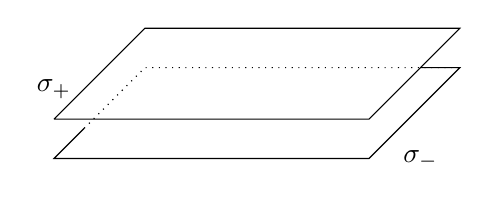
\begin{tikzpicture}{scale = 50em}
        \draw[] (0,0,0) -- (0,0,-3) -- (4,0,-3) -- (4,0,0) -- (0,0,0) node[above = 4]{\(\sigma_+\)};
        \draw[] (0,-.5,-1) -- (0,-.5,0) -- (4,-.5,0) -- (4,-.5,-3) -- (3.5,-.5,-3) node[above = -40]{\(\sigma_-\)};
        \draw[dotted] (0,-.5,-1) -- (0,-.5,-3) -- (4,-.5,-3);
\end{tikzpicture}
\end{wrapfigure}
\noindent Asumiendo que \(\bm{E = \frac{\sigma}{\epsilon_{\textnormal{o}}}}\) es el valor dentro de las dos placas, y \(\bm{d}\) la distancia entre ambas placas, siendo muy pequeña:
\[
        \mathcal{C}  = \frac{Q}{\Delta V} = \frac{Q}{Ed} = \boxed{\frac{\epsilon_{\textnormal{o}S}}{d}}
\]
Posteriormente veremos como, dado un ambiente diferente al vacío, \(\bm{\epsilon_{\textnormal{o}}}\) puede valer otra cosa en función de otra variable.
\subsection{Energía Almacenada en un Condensador}
\noindent Partiendo de que tenemos dos condensadores, uno cargado y otro vacío, ambos con la misma carga pero signos opuestos, las cargas se moverán en función del campo eléctrico que afecta al sistema, redistribuyendo las cargas de forma que cuanta más carga eléctrica se mueva, el potencial eléctrico aumenta proporcionalmente. De esta forma podemos calcular el trabajo, o energía, que se almacena entre las placas:
\[
        \mathrm{d}W = V(q)\mathrm{d}q
\]
\[
        W = \int_{0}^{Q} V(q)\mathrm{d}q = \int_{0}^{Q} \frac{q}{\mathcal{C}}\mathrm{d}q = \frac{q^2}{2\mathcal{C}} \Big|^Q_0 =\frac{Q^2}{2\mathcal{C}}
\]
A veces se denota por la letra \(\bm{\mathcal{\mu}}\), y evidentemente se mide en Julios.
\[
        \boxed{\bm{\mathcal{\mu}} = \frac{Q^2}{2\mathcal{C}} = \mathcal{C}\frac{\Delta V^2}{2}}
\]
Analizandolo de una forma espacial, la energía almacenada no es más que una expresión que relaciona la permitividad del medio y el volumen del campo entre ambas placas:
\[
        \boxed{\bm{\mathcal{\mu}} = E^2 \frac{\epsilon_\textnormal{o}}{2}Sd}
\]
Siendo \(\bm{Sd}\) el volumen entre ambas placas, y \(\bm{\epsilon_\textnormal{o}}\) la permitividad en el vacío, la cual podemos ajustar a cualquier medio.
\subsubsection{Aislantes}
\noindent Al introducir un aislante entre dos placas cualesquiera, \(\bm{\mathcal{C}}\) aumenta, ya que los aislantes se polarizan cuando se someten a un campo eléctrico.\\\\ \textbf{\(\bm{\vec{E}}\) separa las cargas, agrupándolas por su signo y en función de la orientación del propio \(\bm{\vec{E}}\).}
\\\\
Es decir, las cargas se polarizan, en la superficie, y estas tenderán a ser la misma que la polarizada cuanto más cerca estén de la superficie. Pasado un tiempo, la variación de la polarización se invertirá:
\[
        E = \frac{\bm{\sigma_+}-\bm{\sigma_-}}{\epsilon_{\textnormal{o}}}
\]
\subsubsection{Permitivad relativa}
\noindent La permitivad relativa \(\bm{\kappa }\) indica la facilidad con la que la corriente fluye a través de un medio:
\[
        \boxed{\epsilon_\textnormal{R} = \kappa \epsilon_\textnormal{o}}
\]
Siendo \(\bm{\epsilon_\textnormal{R}}\) la permitividad en un medio \(\bm{R}\) y \(\bm{\kappa}\) la permitividad relativa
\subsection{Asociación de condensadores}
\subsubsection{En serie}
\begin{wrapfigure}{r}{6cm}
        \begin{circuitikz}[]
                \draw (-2,0) to[short, l=\(\bm{Q^-}\)] (-1,0)to[C, l_=\(\mathcal{C}\)] (0.5,0)to[short, l=\(0\)] (2,0) to[C, l_=\(\mathcal{C}\)] (3,0) to[short, l=\(\bm{Q^-}\)]  (4,0);
        \end{circuitikz}
\end{wrapfigure}
\noindent \textbf{Por cada uno de los condensadores hay una caída de tensión, pero la intensidad es la misma en todo, por lo que la carga es} \(\bm{cte}\)\\\\
\[
        \boxed{\mathcal{C}_T = \mathcal{C}_{\textnormal{eq}} = \frac{1}{\sum^k_{n=1}\frac{1}{\mathcal{C}_n}}}
\]
\[
        \boxed{V_T = \sum^n_{i=1}V_n}
\]
\[
        \boxed{Q_n = Q_1 = ... = Q_k = cte}
\]

\subsubsection{En paralelo}
\begin{wrapfigure}{r}{1cm}
        \begin{circuitikz}
                \draw (0,0) to[C=\(\mathcal{C}\)] (2,0);
                \draw (0,-2) to[C=\(\mathcal{C}\)] (2,-2);
                \draw (0,-4)  to[C=\(\mathcal{C}\)] (2,-4);
                \draw (0,0)--(0,-6) (2,0)--(2,-6);
        \end{circuitikz}
\end{wrapfigure}
\noindent \textbf{Por cada uno de los condensadores la tensión es la misma, es \(\bm{cte}\), pero la carga no, por lo que la intensidad depende de cada capacitor}:
\[
        \boxed{\mathcal{C}_T = \mathcal{C}_\textnormal{eq} = \sum^k_{n=1}\mathcal{C}_n}
\]
\[
        \boxed{V_n = V_1 = ... = V_k = cte}
\]
\[
        \boxed{Q_T = \sum^k_{n=1}Q_n}
\]